%
\documentclass[11pt]{report}
\usepackage{mathptmx}
\renewcommand{\familydefault}{\rmdefault}
\usepackage[a4paper]{geometry}
\geometry{verbose,tmargin=2cm,bmargin=2cm,lmargin=2cm,rmargin=2cm,headheight=1cm,headsep=1cm,footskip=1cm}
\setcounter{secnumdepth}{3}
\setcounter{tocdepth}{3}
\setlength{\parskip}{\medskipamount}
\setlength{\parindent}{0pt}
\usepackage[numbers]{natbib}
\usepackage{verbatim}
\usepackage{pdfpages}
\usepackage{graphicx}
\usepackage{setspace}
\usepackage[numbers]{natbib}
\usepackage{nomencl}
\usepackage{multirow}
\usepackage{listings}
\usepackage[breakable,skins]{tcolorbox}
\usepackage{float}
\usepackage[titles]{tocloft}
\usepackage{enumitem}
\usepackage{makecell}
\usepackage{amsmath}
\usepackage{hyperref}

\hypersetup{
    colorlinks=true,
    linkcolor=blue,
    urlcolor=blue
    }

%%  Changing indentation  of chapter title in toc
\makeatletter
\renewcommand{\numberline}[1]{%
  \setbox0\hbox{#1\quad}%
  \hb@xt@\wd0{\@cftbsnum #1\@cftasnum\hfil}\@cftasnumb}
\makeatother

% the following is useful when we have the old nomencl.sty package
\providecommand{\printnomenclature}{\printglossary}
\providecommand{\makenomenclature}{\makeglossary}
\makenomenclature
\doublespacing

\makeatletter

%%%%%%%%%%%%%%%%%%%%%%%%%%%%%% LyX specific LaTeX commands.
\providecommand{\LyX}{L\kern-.1667em\lower.25em\hbox{Y}\kern-.125emX\@}
%% Because html converters don't know tabularnewline
\providecommand{\tabularnewline}{\\}
%% A simple dot to overcome graphicx limitations
\newcommand{\lyxdot}{.}


%%%%%%%%%%%%%%%%%%%%%%%%%%%%%% User specified LaTeX commands.
\usepackage{tauthesis}
\usepackage[font={small,bf}, labelfont={small,bf}, margin=1cm]{caption}
\usepackage{titlesec}
\newcommand{\hsp}{\hspace{20pt}}

\titleformat{\chapter}[hang]{\Huge\bfseries}{\thechapter\hsp}{0pt}{\Huge\bfseries}

\Title{\textbf{Portable RF System for Network Bridging}}
\Author{\textbf{Tigran Tadevosyan}
\\ \vspace{0.5cm}
Supervised by: Vahagn Mkhitaryan }
\Year{May 2023}
\Supervisor{Vahagn Mkhitaryan}
\Department{Department of Computer Science}
\Degree{Bachelor in Computer Science}
% \Degree{Doctor of Philosophy}

\makeatother

\usepackage[english]{babel}
\begin{document}

\prelimpages


\titlepage



\chapter*{Abstract}

The following system facilitates two-way radio communication between devices with a physical network interface. Although it can be used to directly connect two devices with network capabilities, it can also bridge subnetworks. As it provides DHCP server capabilities, it is a plug and play system. The components of the system are portable, requiring low power usage, and can provide a connection in ranges over 10 km, so it can be a powerful tool for utilizing myriad networking technologies. 

%\tableofcontents{}
\tableofcontents

\textpages

\listoffigures

\listoftables

\printnomenclature{}

%\footnote{Split the thesis into separate chapters. Use \textbackslash{}include mode to include the separate files.}


\chapter{Introduction}

% \section{Motivation}
% In the span of the past three decades, the internet has blossomed into an indispensable facet of our daily existence. From the ubiquitous presence of smartphones, which have become synonymous with connectivity, to the unexpected convergence with unconventional devices such as internet-connected cow milking apparatus, the internet has woven itself intricately into the fabric of modern life. This project embarks upon a daring experiment, seeking to address a profound question: can a student from the year 2023 harness the ingenuity possessed by the geniuses of the past half-century, and engineer a fully functional communication network, all the while leveraging on the readily available hardware and the wealth of knowledge graciously bestowed upon him by these very pioneers?

\section{Structural Overview}

\begin{figure}[H]
\begin{center}
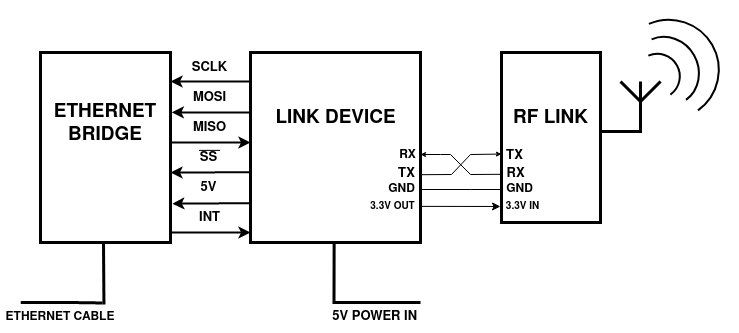
\includegraphics[width=1\textwidth]{schematic-diagram}
\end{center}
\caption{Schematic Diagram of a Single Agent.}
\label{fig-pin}
\end{figure}

In the current form, the system is designed so as to facilitate communication between two agents. Both have three main hardware components: Link device, Ethernet bridge, and RF link. The main computational unit, which handles most of the data processing, is the Link device. The Ethernet bridge is used to provide Ethernet connectivity to the Link device, as it misses the necessary hardware interface. The Ethernet bridge is running stock firmware with no addition software written for it. 
The connection between Link device and Ethernet bridge is facilitated via SPI. The last component is the RF link, the sole purpose of which, is to perform the data transmission over RF. The communication between Link device and the RF link is maintained via UART. The functionality of RF link is abstracted away, so the Link devices are operating as if they are directly connected to each other. Even though there is only one Ethernet interface on both agents, both sides can provide connectivity to multiple network user devices if they are connected through a network switch or hub. Currently, we have an arbitrary limitation of 16 clients on each side, but even fewer number of clients would not be able to use the network, because of the modest network throughput.

% \newpage

As the purpose of our system is Network Bridging, data from one end interface to another passes over 6 components:
\begin{enumerate}[nolistsep]
    \item Transmitter side's Ethernet bridge,
    \item Transmitter side's Link device,
    \item Transmitter side's RF link,
    \item Receiver side's RF link,
    \item Receiver side's Link device,
    \item Receiver side's Ethernet bridge.
\end{enumerate}

This causes a demand for packet nesting structure. Figure \ref{packet-nesting} illustrates that structure.

\begin{figure}[H]
\begin{center}
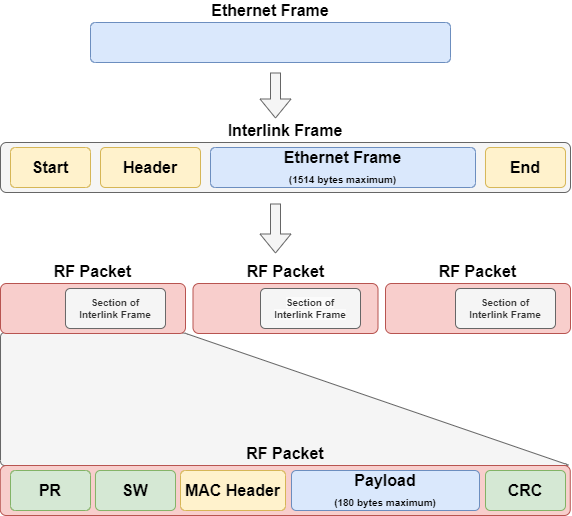
\includegraphics[width=0.8\textwidth]{packet-nesting.png}
\end{center}
\caption{Overview of System's Packet Nesting Structure.}
\label{packet-nesting}
\end{figure}

The whole source code of the project is available on \href{https://github.com/Tigran-teq-Tadevosyan/TIR}{Github} \footnote{https://github.com/Tigran-teq-Tadevosyan/TIR}.


\section{Hardware}
\begin{enumerate}[nolistsep]
\item PIC32MZ DA Curiosity Development Kit (Link device),
\item TI Lunchpad kit with CC1312R1 MCU	(RF link),			
\item JESSINIE board with W5500 embedded Ethernet controller (Ethernet bridge),
\item Rigol DS1102E Digital Oscilloscopes \footnote[1]{For debugging purposes and for some of the screenshots included in this report.}.
\end{enumerate}

\section{Software}
\begin{enumerate}[nolistsep]
\item MPLAB X IDE v6.05,
\item MPLAB IPE v6.05,
\item MPLAB XC32 Compiler v4.21,
\item Code Composer Studio v12.3.0,
\item GCC v9.2.1 (Linaro) \footnote[2]{Version for AMD64 to ARM cross-compilation.},
\item TI Lunchpad kit with CC1312R1 MCU,
\item Wireshark v12.3.0 \footnote[3]{For debugging purposes and for some of the screenshots included in this report.}.
\end{enumerate}
\chapter{Link Device}
For the Link Device we have decided to use the PIC32MZ DA Curiosity development kit from Microchip with PIC32MZ2064DAR176 MCU on it. It is powerful enough for our usage and has all the necessary connectivity for the project, except for an Ethernet interface, for which we have used the W5500 chip from WIZnet.

\begin{figure}[htp]
\begin{center}
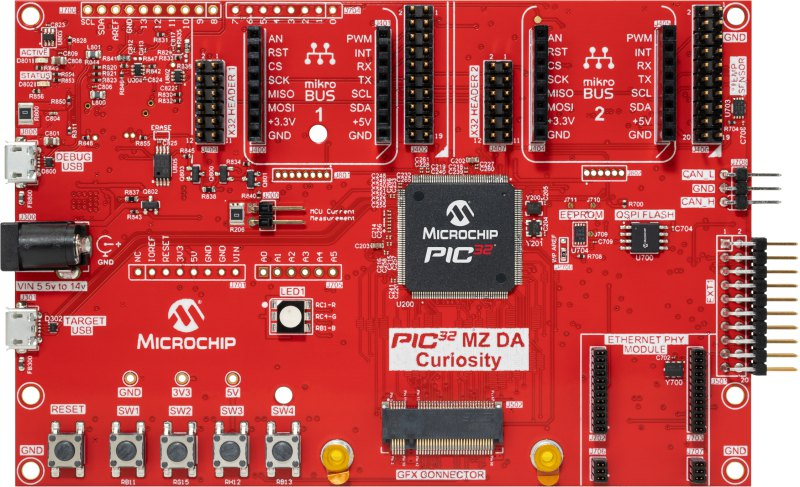
\includegraphics[width=0.8\textwidth]{PIC32MZ-DA-curiosity}
\end{center}
\caption{Top View of PIC32MZ DA Curiosity Development Kit}
\label{pic32da-curiosity-top-view}
\end{figure}

\begin{table}
\centering
\caption{Technical Specifications of PIC32MZ DA Curiosity \cite{pic-datasheet}}
\label{table1}
\begin{tabular}{|l|l|}
\hline 
MCU Model & PIC32MZ2064DAR176 \\ \hline
MCU Architecture & 32-bit MIPS \\ \hline
MCU Max Frequency & 200 MHz \\ \hline
Program Memory Size & 2048 KB \\ \hline
SRAM & 640 KB \\ \hline
\end{tabular}
\end{table}

\section{Interlink Protocol}

In order to facilitate efficient internal communication among Link devices while simultaneously tunneling external traffic, it is imperative to establish a clear distinction between service packets and forwarding requests. For this purpose, linked devices are using a so-called “Interlink” protocol. 

\begin{table}
\centering
\caption{Interlink packet structure}
\label{interlink-pkt-struct}
\begin{tabular}{|p{1in}|p{1.5in}|p{2in}|} \hline 
\multirow{3}{*}{Header} & Start Delimiter & {4 bytes} \\ \cline{2-3}
 & Payload Length & 2 byte unsigned integer \\ \cline{2-3}
 & Message Type & 1 byte \\ \cline{2-3} \hline
 \multicolumn{2}{|c|}{Payload} & Up to 1514 bytes \\ \hline
 \multicolumn{2}{|c|}{End Sequence} & 2 bytes \\ \hline
\end{tabular}
\end{table}

As the Interlink packets are being transmitted over RF, data losses are eminent. Moreover, the packets can be split between two time slots, or the same time slot can carry information of two packets (the idea of the times slots is covered in the RF Link section). To avoid this problem, we must be able to identify the start and the end of the Interlink packets. We do so by starting every packet with a 4 byte start delimiter that is represented by an improbable combination of symbols {0x26, 0x24, 0x26, 0x24} (“\$ \& \$ \&” in ASCII) and ends with a 2 byte sequence of {0x04, 0x04} (two end of transmission symbols in ASCII). 

During data reception when encountering a start delimiter, we make sure that at the end of the payload (calculated by the payload length) an end sequence is present. If not, we drop two bytes and search for the next start delimiter in the sequence. Through this procedure we ensure that a data loss in one packet would not result in inclusion of the next packet’s beginning in this one, corrupting both packets. Although this procedure is designed to address the unreliability of RF, we include this in Interlink, as this also would help with the unreliability of the UART, which is less of an issue, however errors are still possible on relatively high baud rates (230400), especially at the beginning of the serial transmission.

The start delimiter is followed by a 2 byte representation of the packet payload length as a little-endian unsigned integer. The biggest payload we intend to encapsulate in an interlink packet is the Ethernet frame, which consists of the destination address (6 byte), the source address (6 byte), the Ethertype (2 byte) and the payload (at most 1500 byte as we do not support jumbo frames used in high performance networks), so 2 bytes will suffice.

The last byte in the header indicates the message type, possible values of which are listed below:
\begin{itemize}[nolistsep]
    \item HANDSHAKE\_REQUEST,
    \item HANDSHAKE\_OFFER,
    \item HANDSHAKE\_ACK,
    \item FORWARDING\_TABLE\_ADDITION,
    \item FORWARDING\_TABLE\_REMOVAL,
    \item FORWARDING\_REQUEST.
\end{itemize}

The first five message types are for the service packets, intended for the internal communication between the Link devices, and the last one is for the frame forwarding request, that will be discussed later. The service packets are used to accommodate the handshake procedure and carry out the forwarding table synchronization.

\section{Handshake Procedure}

Every device in our network has a dedicated role. Upon power on, the device is assigned UNDEFINED\_ROLE, and to acquire a role, it must go through the handshake procedure. Currently, we only have 2 designated roles (DHCP\_SERVER1 and DHCP\_SERVER2), however, the procedure is designed to be relatively easily extendable to more roles and a higher number of agents in the network. Throughout the handshake procedure, there are three possible states that the agent can be in: HANDSHAKE\_UNINTIALIZED, WAITING\_ROLE\_ACK, HANDSHAKE\_FINISHED.  Upon power on, the Link device sends a “HANDSHAKE\_REQUEST” message with an empty payload signaling its readiness for a handshake. Moreover, a request timeout is generated in the range of 250 to 1000 ms using a pseudo-random number generator, which was seeded with the value in 32 bit “DEVSN0” register (DEVSN0 to DEVSN3 registers contain a unique serial number of the device \cite{pic-datasheet}). The device continues to repeatedly send out requests with the aforementioned timeout delay for 10 times, after which, if no valid response is received, it assigns itself a role. The timeout duration is calculated randomly to avoid collisions of requests sent by the other agents. Even in the scenario when the agent A gets a randomly generated number \(\Delta t_A\) as the timeout delay, and the agent B, being booted up at time \(t_B\)  starting from boot time of the first device, gets a timeout delay of \(\Delta t_B = \Delta t_A - t_B\), resulting in the two requests being transmitted at the same time causing a collision, this would still not be an issue as on the next repeat of either agent’s “HANDSHAKE\_REQUEST” it would reach the peer. Upon receiving a “HANDSHAKE\_REQUEST” packet, two scenarios can occur. First, if the agent-receiver has no role assigned to it yet, it will assign a role to itself and will send an “HANDSHAKE\_OFFER” message to the peer. In our case it would assign the role of “DHCP\_SERVER1” to itself and offer the “DHCP\_SERVER2” role to peers. In the second scenario, if the agent-receiver already has an assigned role, it would just offer the other role to the peer by again sending a “HANDSHAKE\_OFFER” message, which contains the offered roles in message payload.
After sending the “HANDSHAKE\_OFFER” message, the agent proceeds to the “WAITING\_ROLE\_ACK” handshake state. As in the case of the “HANDSHAKE\_REQUEST” messages, there is another timeout generated with a random number generator, and we again repeat the “HANDSHAKE\_OFFER” a maximum of 10 times. If no acknowledgement message is received during these repetitions, the agent rolls back into “HANDSHAKE\_UNINTIALIZED” state.
Upon receiving a “HANDSHAKE\_OFFER” message, if the agent is in the state of “WAITING\_ROLE\_ACK” or “HANDSHAKE\_FINISHED”, if the roles in payload coincide with the roles it has it has registered, it respond with a “HANDSHAKE\_ACK” message. In the case of agent-receiver being in “WAITING\_ROLE\_ACK” state, it performs same procedure, after which it also start the DHCP server (covered later) with agreed roles. If the roles do not match or the agent-receiver is in “HANDSHAKE\_UNINTIALIZED” state, it just ignores the message.
Upon receiving a “HANDSHAKE\_ACK” message if the agent is in the state of “WAITING\_ROLE\_ACK” and the roles in the message match, the current registered roles of agent-receivers starts the DHCP server with the agreed roles, otherwise it just ignores the message. 
It is important to mention that in cases when receiver-agent is in the state of “HANDSHAKE\_FINISHED” and it receives a “HANDSHAKE\_OFFER” or “HANDSHAKE\_ACK” message with roles matching to his role assignments he also sends ”FORWARDING\_TABLE\_ADDITION” messages for all his valid DHCP bindings (covered later).

\section{DHCP Server}

The Open Systems Interconnection model (OSI model) is a widely accepted conceptual model that “provides a common basis for the coordination of standards development for the purpose of system interconnection.” \cite{OSI} It consists of the following 7 layers: Physical, Data Link, Network, Transport, Session, Presentation, and Application. The first layer, the physical layer, is the layer that describes the physical connection between devices, meaning that it describes the standard procedure of the transmission through the given medium. In this project we are focusing on IEEE 802.3 (Ethernet). 

\begin{figure}[htp]
\begin{center}
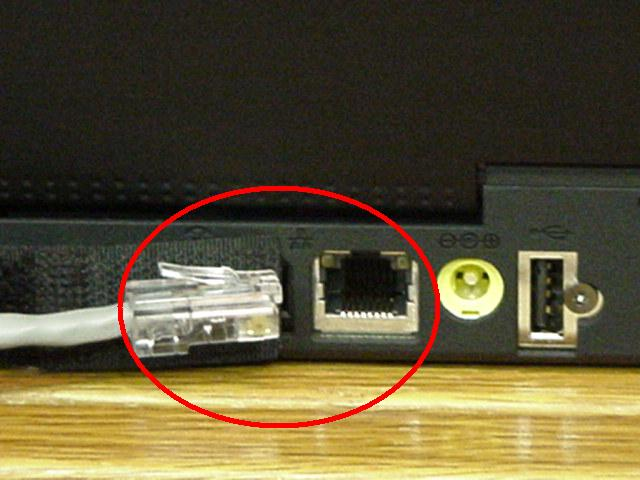
\includegraphics[width=0.8\textwidth]{ethernet-port}
\end{center}
\caption{Ethernet Port}
\label{ethernet-port}
\end{figure}

The second, data link layer, describes the protocols by which data is transferred between nodes on a network across the physical layer \cite{data-link-layer}. IEEE 802.3 standard also describes the layer 2 communication protocol, commonly referred to as just Ethernet. Data is transmitted by so called Ethernet frames, which have the following structure:

\begin{figure}[htp]
\begin{center}
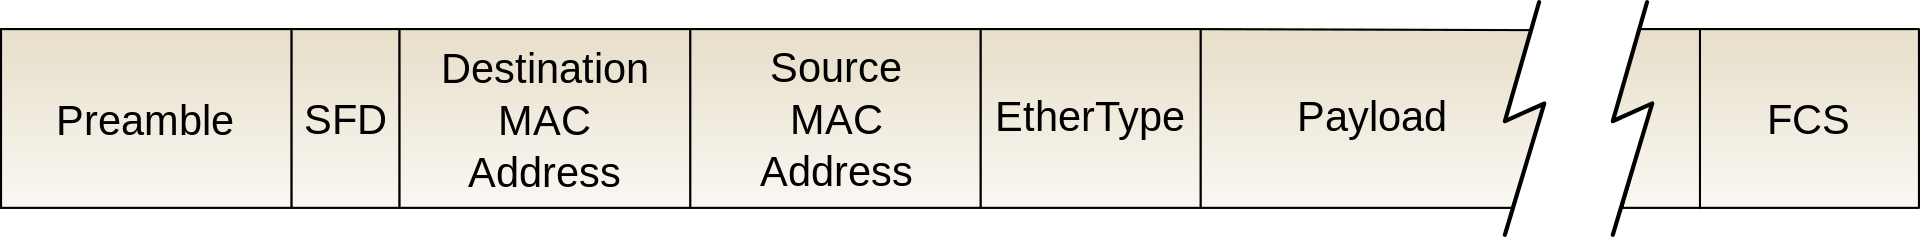
\includegraphics[width=1\textwidth]{Ethernet-frame}
\end{center}
\caption{Ethernet Port}
\label{ethernet-port}
\end{figure}

\begin{enumerate}[nolistsep]
    \item Preamble - The preamble consists of a 56-bit (seven-byte) pattern of alternating 1 and 0 bits, allowing devices on the network to easily synchronize their receiver clocks, providing bit-level synchronization, 
    \item SFD - The eight-bit (one-byte) value that marks the end of the preamble,
    \item Destination MAC address,  
    \item Source MAC address,
    \item EtherType - The type message in the payload of the frame,
    \item Payload - The data that is carried inside the frame,
    \item FCS - A four-octet cyclic redundancy check (CRC) that allows detection of corrupted data within the entire frame as received on the receiver side.
\end{enumerate}

Every network interface controller (NIC) has a unique MAC (Media Access Control) address assigned to it by the manufacturer. It consists of 6 octets, out of which the first three are given to the NIC manufacturer. Devices use these addresses to communicate in local area networks (LAN). 

The next is the network layer, which is responsible for packet forwarding including routing through intermediate routers \cite{data-link-layer}. Internet protocol (IP) is one of the protocols of the network layer that most of the internet runs on. There are two major versions of IP, Internet Protocol Version 4 (IPv4), and its successor Internet Protocol Version 6 (IPv6). In the IPv4 protocol the IP address is a 4 byte number that is usually represented by four consecutive numbers in the range of 0-255 separated by dot (for example 192.1.0.7). An IPv6 address is represented as eight groups of four hexadecimal digits, each group representing 16 bits The groups are separated by colons (for example 2001:0cc8:87a3:0000:0000:8a4e:f270:7a3c) \cite{ipv6-arch}. These addresses are used for the routing purposes, meaning that routing nodes forward the IP packets via their IP addresses. Even though most of the internet infrastructure already supports IPv6, most of the internet still runs predominantly on IPv4. IP packets are nested inside layer 2 packets, mostly Ethernet or Point-to-Point Protocol (PPP). Below is the structure of IPv4 package: 

\begin{figure}[htp]
\begin{center}
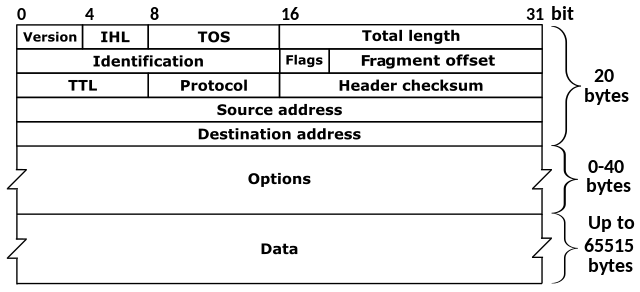
\includegraphics[width=1\textwidth]{IPv4-Packet.png}
\end{center}
\caption{IPv4 Packet structure}
\label{ethernet-port}
\end{figure}

As this is not a crucial element of our project, there is no need to elaborate on this structure in further detail.
Packets of the higher layers of the OSI model are encapsulated within the IP packets, and if the MAC addresses are assigned during the manufacturing of the NIC, the IP addresses are dynamically assigned within the network when they are connected to it. The role of the IP assignment is performed using the Dynamic Host Configuration Protocol (DHCP) by DHCP server. In the case of the home networks this role is usually performed by the router. However, as there might not be a DHCP server in our network,  to be able to make use of the IP and all the higher level protocols we have two solutions. First is statically configuring every single device in the network or our Link devices should perform the role of the DHCP server. As we want to make the process of connecting devices to our network plug and play, we had to go with the second option. DHCP is an application layer (layer 7) protocol, meaning it must be encapsulated as a payload of a lower layer protocol’s packet to be transmitted over the network. In the case of the DHCP, it is encapsulated inside User Datagram Protocol (UDP), which itself is a transport layer (layer 4) protocol, which in its turn is encapsulated inside IP packet (IPv6 in case of the DHCPv6 and IPv4 in case of the DHCPv4), which is finally encapsulated in the ethernet frame. 

\begin{figure}[htp]
\begin{center}
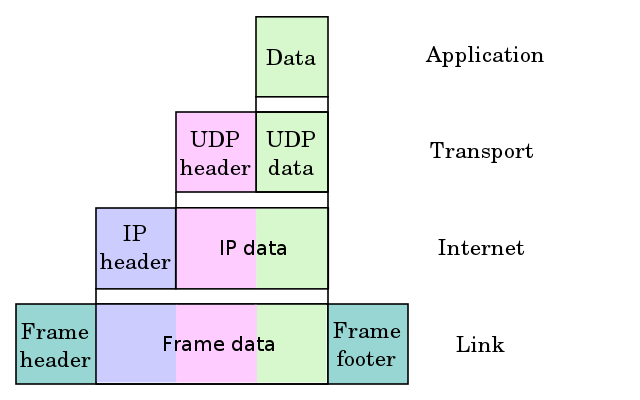
\includegraphics[width=0.7\textwidth]{UDP-encapsulation}
\end{center}
\caption{Network Message Encapsulation}
\label{ethernet-port}
\end{figure}

This way, if we want to be able to serve DHCP messages, we must be able to work with all these protocols mentioned above. We have taken two main limitations not to overly sophisticate the program at this stage. As virtually any device supports IPv4 and DHCPv4, we only support those versions, and as the Maximum Transmission Unit (MTU) in our network is plenty enough to facilitate the biggest possible DHCP message (548 bytes in case of DHCPv4), we do not support IP packet fragmentation.

As our DHCP message is going to be encapsulated inside a UDP packet, let us briefly go over the structure of its header. It consists of four fields: source port, destination port, length, and checksum. Each of the fields are 2 bytes long. In our case, the DHCP server listens to its UDP port number 67 and the client listens to the UDP port number 68, meaning that messages sent from the client to the server must have destination port set to 67 and source port to 68, or vice versa for the server to client communication. Moreover, we skip the checksum calculation also as it is not mandatory in the case if the UDP message is encapsulated inside an IPv4 packet, so this field is always set to 0s.
DHCP operations fall into four phases: server discovery, IP lease offer, IP lease request, and IP lease acknowledgement \cite{book-computer-networks}. Below is an illustration of a typical DHCP transaction for IP address acquisition.

\begin{figure}[htp]
\begin{center}
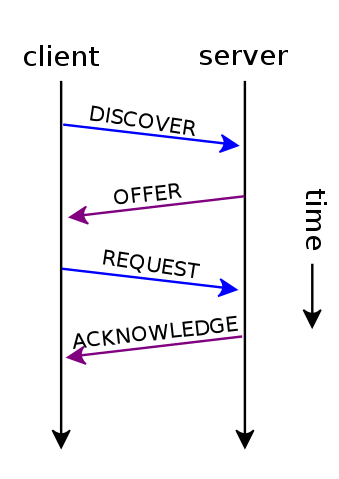
\includegraphics[width=0.3\textwidth]{DHCP_session}
\end{center}
\caption{Illustration of Typical DHCP Session}
\label{ethernet-port}
\end{figure}

The DHCP session usually starts with the client sending a DHCPDISCOVER message using the destination address 255.255.255.255 (broadcast address). The DHCP client may also include the IP that it is requesting and other options like request for a subnet mask, router address, Domain Name Server (DNS) address, etc. When a DHCP server receives a DHCPDISCOVER message from a client, it responds with a DHCPOFFER message, usually using a broadcast address too. After receiving a DHCPOFFER message client would respond with a DHCPREQUEST message with requested IP address in it and if DHCP servers confirms the assignment by sending DHCPACK message. We wouldn't explor the exact details of the protocols, which can be found here (SOURCE HERE), as it is out of this reports scope, but here are a series of screenshots of Wireshake (network packet sniffing software) of steps in the DHCP session performed via our DHCP server.

\begin{figure}[htp]
\begin{center}
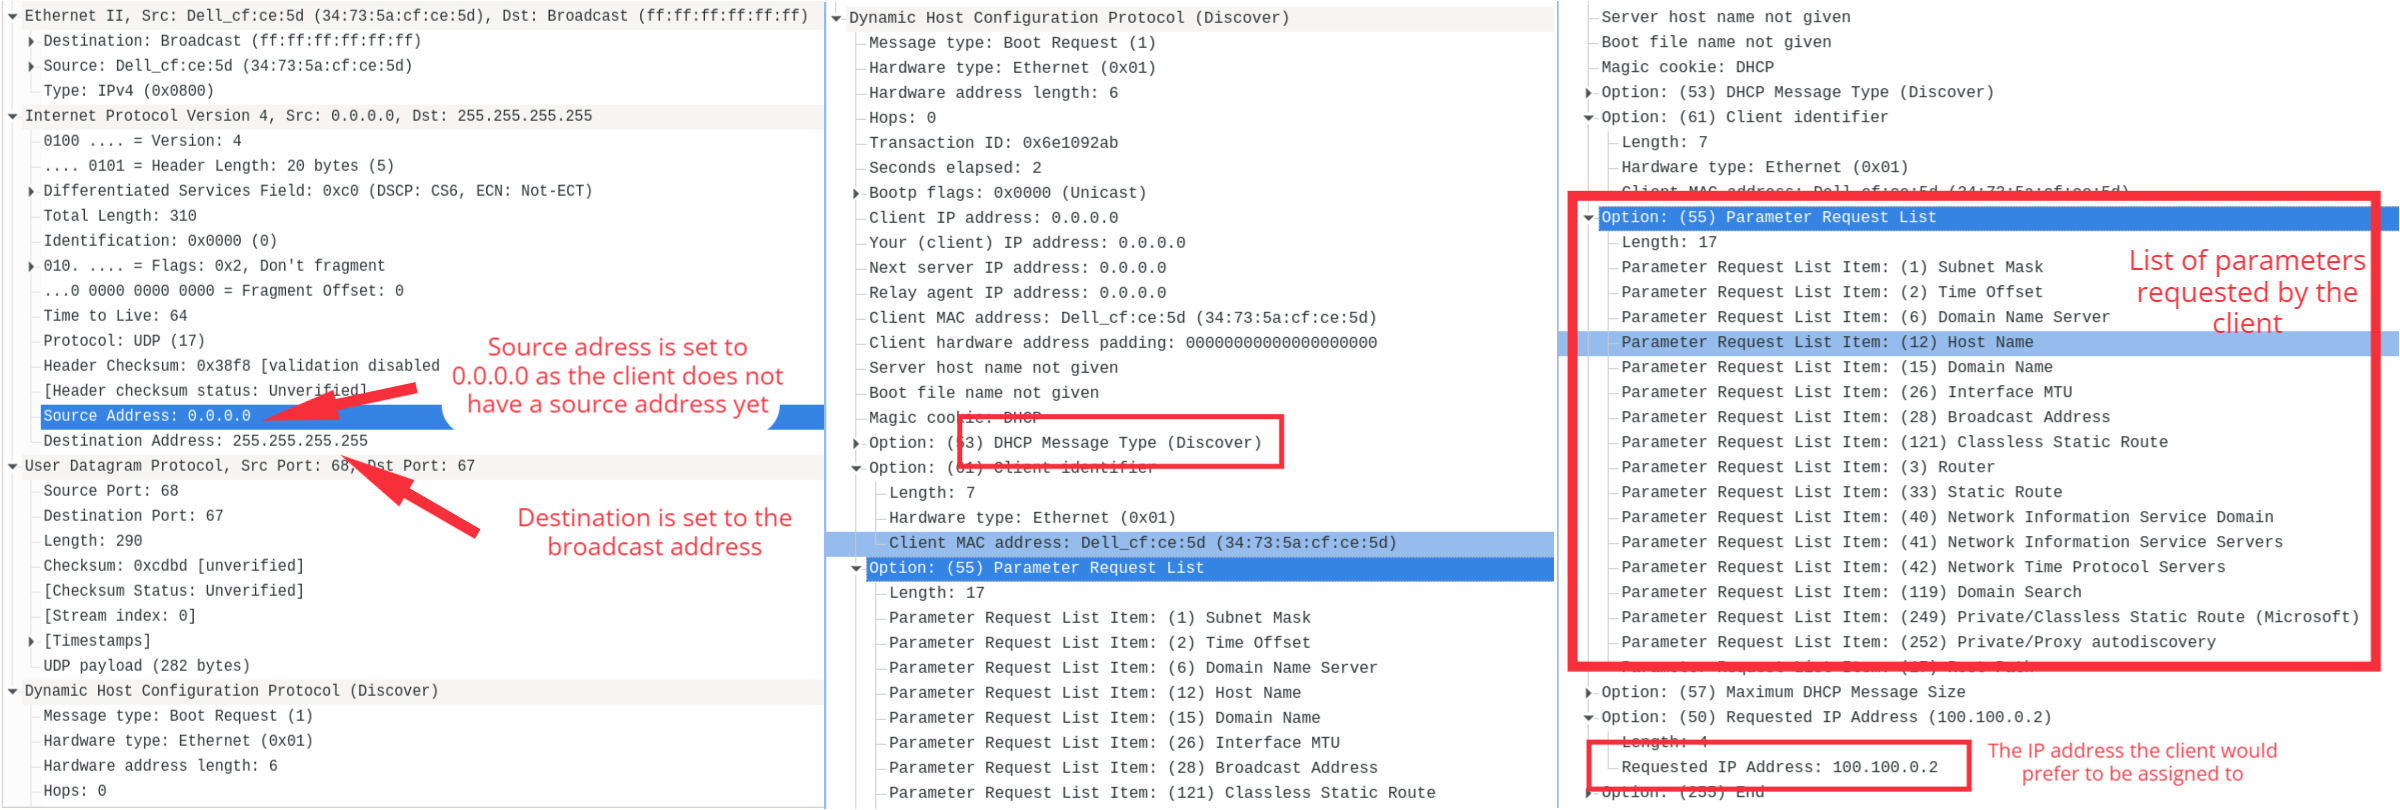
\includegraphics[width=1.1\textwidth]{DHCP-Discovery.png}
\end{center}
\caption{Screenshots of DHCP Discovery Packet.}
\label{dhcp-discovery}
\end{figure}

\begin{figure}[htp]
\begin{center}
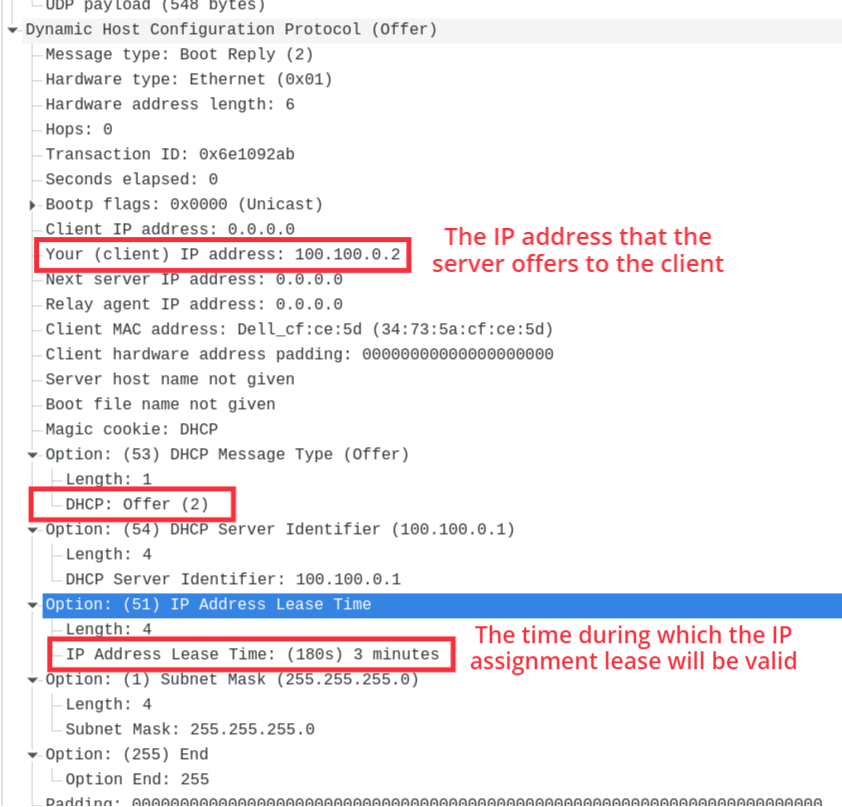
\includegraphics[width=0.7\textwidth]{DHCP-Offer.png}
\end{center}
\caption{Screenshots of DHCP Offer Packet.}
\label{dhcp-offer}
\end{figure}

\begin{figure}[htp]
\begin{center}
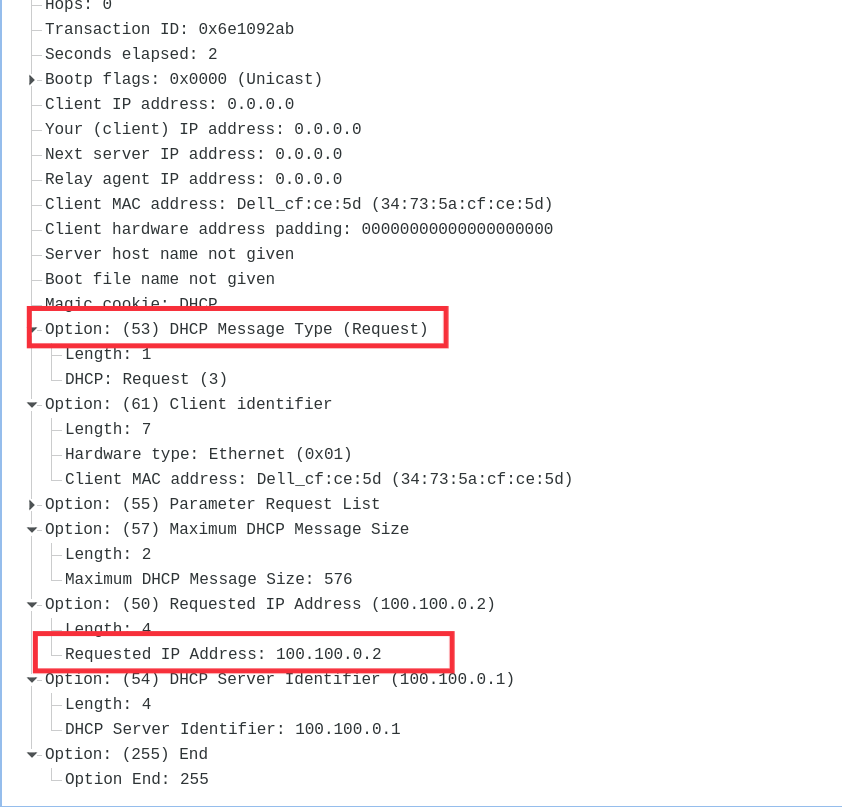
\includegraphics[width=0.7\textwidth]{DHCP-Request.png}
\end{center}
\caption{Screenshots of DHCP Request Packet.}
\label{dhcp-request}
\end{figure}

\begin{figure}[htp]
\begin{center}
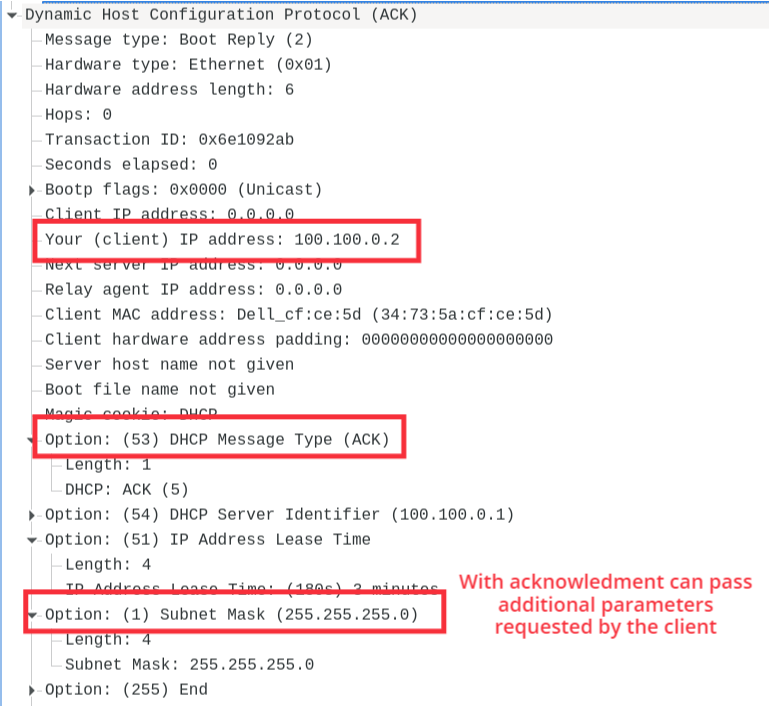
\includegraphics[width=0.7\textwidth]{DHCP-Ack.png}
\end{center}
\caption{Screenshots of DHCP Acknowledgment Packet.}
\label{dhcp-ack}
\end{figure}

\newpage

After the client is assigned the IP address, it sends additional DHCPREQUEST messages (without prior DHCPDISCOVER message) with a certain timeout before its lease time has expired, so it would not be removed from DHCP bindings of the server. Moreover, our Link devices are communicating between each other with Interlink message types of “FORWARDING\_TABLE\_ADDITION” and “FORWARDING\_TABLE\_REMOVAL” to notify in the addition and removal of the DHCP bindings in their list, so the other servers know to what IPs and MAC addresses the incoming messages should be forwarded and which should be dropped. 
Link devices are set up to have an IP address of 100.100.0.1 with a subnet mask of 255.255.255.0.  So we can assign IP addresses in the range of 100.100.0.2 to 100.100.0.254, as 100.100.0.1 is assigned to us and 100.100.0.255 is reserved for broadcast. The ranges of IP addresses in which individual Link devices are allowed to assign is based on their role. In our case as we have just two roles, the “DHCP\_SERVER1” would give out IP addresses in the range of 100.100.0.2 to 100.100.0.100, and “DHCP\_SERVER1” would give out IP addresses in the range of 100.100.0.101 to 100.100.0.254. The lease time is set to be 3 minutes and we perform maintenance (for removal of expired DHCP binding) every 5 seconds. 

\section{Efficient Packet Queue Structure}

During normal operation most of the data traffic that Link device receives from Ethernet bridge is going to be pass to RF link, while most of the traffic received from RF link is going to be passed to Ethernet bridge. This means that designing an efficient algorithm that abstains from unnecessarily coping memory segments in memory would provide a reduced latency and better performance for our system. On both RF link and Ethernet bridge side we are using static buffers which we are going to discuss in subsequent sections, but for use to be able to operate in such fashion have to have some method of keeping track of packets in the buffers.  

\begin{figure}[htp]
\begin{center}
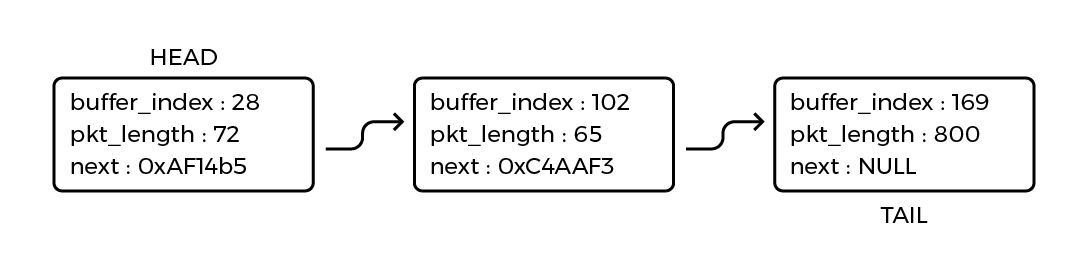
\includegraphics[width=0.8\textwidth]{queue-pkt-struct}
\end{center}
\caption{Illustration of Packet Queue.}
\label{pkt-queue-stuct}
\end{figure}

Figure \ref{pkt-queue-stuct} illustrates the inner workings of our packet queue. We have decide to implement it based on a linked list, which means that we would have to allocate memory for each node dynamically, but also gives us the ability to omit a limitation on the number of packets we can track. Taking into consideration the fact that each node take up just 8 bytes in memory and the packet data is located in static buffers the trade off beneficial. This way we are able to read received data into a buffer, analyze it, and then forward it from the same memory location if there would be a need for it.  

\section{Connection to W5500}

As our PIC32MZ DA Curiosity development kit does not have the hardware interface necessary for Ethernet connection, we have to rely on additional hardware to achieve that. For that purpose, we have decided on an integrated board from JESSINIE with the WIZnet W5500 embedded Ethernet controller on it.

\begin{figure}[htp]
\begin{center}
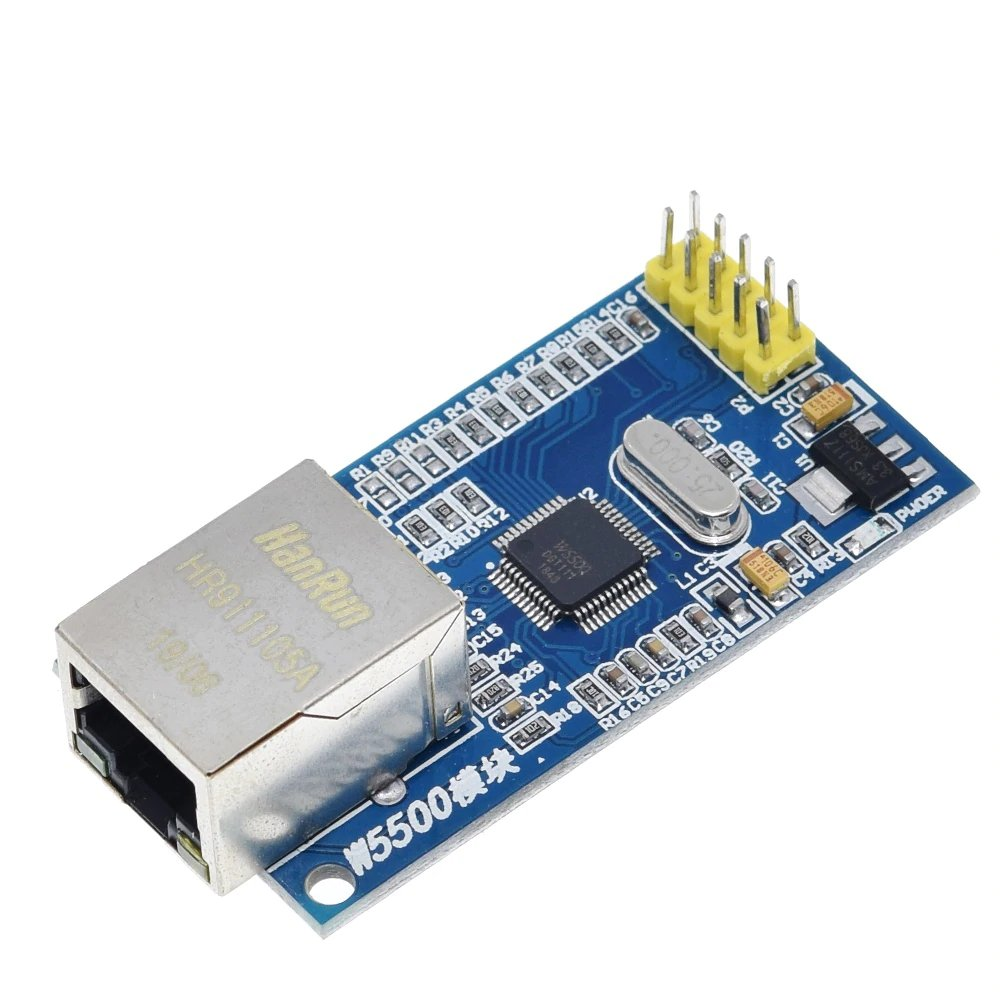
\includegraphics[width=0.5\textwidth]{w5500}
\end{center}
\caption{WIZnet W5500 embedded Ethernet controller.}
\label{ethernet-port}
\end{figure}

The connection between our Link device and the W5500 is maintained using Serial Peripheral Interface (SPI). Naturally Link device is operating in “master” mode and the W5500 is operating in “slave mode”. The SPI clock frequency is set at 20 MHz. This is way lower than 80 MHz, which is the maximum frequency the chip is rated to work in. We assume the problem lies in the bad quality of the cables that we used and the fact that in our prototype we use cables to connect the W5500 to PIC32 controller, which introduce parasitic resistance and capacitance on SPI lines. However, we did not continue to investigate this issue further as higher SPI frequencies would not result in better performance, because even at 20 MHz it is not the bottleneck of our system.
We are using the official driver library from WIZnet to communicate with the chip. We initialize the W5500 with network configuration described in table \ref{w5500-net-conf}.

\begin{table}
\centering
\caption{W5500 Network Configuration}
\label{w5500-net-conf}
\begin{tabular}{|l|l|}
\hline 
MAC address & A5:E6:38:61:B8:71 \\ \hline
IP address & 100.100.0.1 \\ \hline
Subnet mask & 255.255.255.0 \\ \hline
\end{tabular}
\end{table}

W5500 supports a total of 8 “sockets” which support various modes, but we are using the so-called “MACRAW” mode, because it provides with maximum control over the socket. Only the socket 0 supports “MACRAW” mode, so that is the socket we are going to use. Although we are losing on performance by not utilizing the majority of functionalities of the chip, in our case we have no other choice as we need to process the raw ethernet frames, and the “MACRAW” mode is the only one that provides us with that ability. The only hardware feature we are using is hardware level IPv6 blocking, as we are not intending to support them in the scope of this project \cite{w5500}.

The W5500 has a combined memory of 32 KBs, half of which is for the RX buffer and the other half for the TX buffer. As we are only utilizing one socket, we fully assigned the whole memory of both the buffers to that socket. During the initialization of the socket we set two interrupts in its interrupt mask, which are reception interrupt and transmission interrupt. Our initial plan of enabling a callback on the interrupt pin of this chip quickly fell apart, as we understood that the library provided by WIZnet is written in a way that makes working with the chip in such a manner really inconvenient. So we decided to operate the SPI in blocking mode and handle interrupts in the program execution loop. In fact, later we have discovered that the chip is behaving strangely, as it gives out a reception interrupt, when there is no data available to read and sometimes the opposite occurs, so we don't even pay attention to that status and just read the number of available data on every iteration. The same cannot be said about the sent status, as it seems to work fine.

In case of data reception we are going to use the data structure described in section 2.4 and a 30 KB static buffer. 

\begin{figure}[htp]
\begin{center}
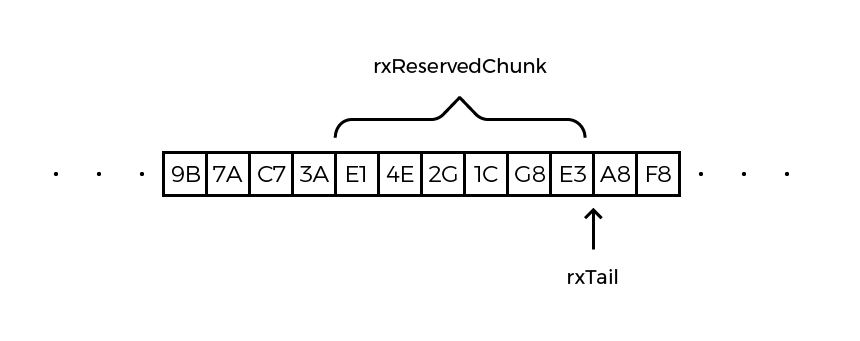
\includegraphics[width=0.7\textwidth]{macraw-rx-buffer}
\end{center}
\caption{RX Buffer of MACRAW Socket.}
\label{macraw-rx-buffer}
\end{figure}

As it is ilustrated in the figure \ref{macraw-rx-buffer}, we only need to keep track of two values: 
\begin{enumerate}[nolistsep]
    \item rxReservedChunk - the length of reserved chunk, which is located directly before the rxTail,
    \item rxTail - the position of reserved chunk's end.
\end{enumerate}

If there is any data that must be read from W5500, we just reserve that amount of space at the rxTail position of our static buffer and return the pointer to the reserved section for data to be written there. During the execution loop of our program we analyze the contents of the reserved chunk and perform one of the following procedures: 
\begin{itemize}[nolistsep]
    \item If the received frame is a DHCP message, we respones to it accrodingly.
    \item If the received frame eather contains an IPv4 or ARP packet, and the MAC of IP address in the packet headers match any one of forwarding table entries we received from pair agent, we enqueue that packet in the aforementioned queue structure, for the data to later be passed to RF link.
\end{itemize}
It is important to mention on every data reception from Ether bridge, before reserving memory check if the reservation of this data would cause an override of data packet that was still not forwarded to RF Link, if so we abstain from reading that data until enough memory is freed in our buffer\footnote{This could potentially cause an overflow of W5500's inner rx buffer, resulting in a data loss, which is inevitable in case our modest throughput}. Last important remark is that as want to our data to be directly transmitted from the memory location we have read it to, we are forced to work with continues blocks of memory, meaning the circular buffer can't wrap at the end of the buffer and spit the frame into to separate memory chunks. This means that if the remaining amount memory left at the end of the buffer is not enough for reception, we have to return to the start of the buffer and left the end unutilized. Moreover, a scenario might occur where we have some yet not analyzed data in reserved chunk right before the rxTail, which might contain the beginning of a frame we are about to read from Ethernet bridge. This will again cause a frame fragmentation which forces us into moving that reserved chunk to the beginning of the buffer and reserving new chunk at the end of that one to ensure continuity of frames.

\section{Link Device UART Connection}

For the connection to RF link we have used UART. It may seem that using SPI to achieve higher speeds would be a better approach. Reason for not doing so is that setting up MCU's as "slave" devices in configurations similar to ours is tedious and in our case unnecessary as we are not "bottle-necked" by the Link device to RF link's  communication speed, but, as it would become apparent later, by the processing power of the RF link MCU's. The UART is running at 230400 bauds per second.

To reduce the amount of processing resources we dedicate to UART servicing we have have made use of a feature that our MCU supports called \textbf{Direct Memory Access (DMA)}. Its a hardware subsystems that can access main system memory and copy memory around independently of the processing unit. Our MCU's architect is realize is such a way that system memory is divided into two sections: \textbf{KSEG0} and \textbf{KSEG1}. The memory in \textbf{KSEG0} cacheable and \textbf{KSEG1} \cite{pic-datasheet}. This in turn means that operations in \textbf{KSEG0} can be optimized by the MCU. Obviously, the use of L1 cached make it impossible for DMA to work with \textbf{KSEG0} memory as it work separately from processing unit. This forces us to use memory located in \textbf{KSEG1} for the static buffers use for UART communication. Moreover, as we want to transmit the data received from Ethernet bridge to RF link without copying it we have to allocate it's buffer in \textbf{KSEG1} section too. As the data is sent to RF core directly from the static buffer used for Ethernet bridge reception, we do not need to keep a separate buffer for transmission, but just keep track of packets we must pass to RF link with the use of Packet Queue data structure, and free them after they are sent. The reception is not that straightforward, as we do not know the exact amount of data we are going to receive, so we are unable to configure DMA channel to copy that amount of data to reception buffer from UART register. The simplest solution would be to perform just 1 byte coping operations, but this will kill the purpose of DMA as we would get reception completion callbacks on every byte making this process very inefficient. The reason why we can't just increase number of bytes to be received, before reception interrupt is raised, is that if for example we have a reception block size of 100 bytes and we have received 99 byes of data, the interrupt would not be raised until 1 more byte is received. This may cause a lot of issued as for example that 99 bytes may contain acknowledgement message that receiving side is wait to send more data. Or even in our case "HANDSHAKE\_REQUEST" is just 7 bytes long, so there must be 15 of them received for the threshold to be received. One possible solution could be adding padding to messages so they are multiple of block size, but because of the unreliable nature of RF we could loose some data causing the aforementioned issues. To solve this we have check the \textbf{DCH1DPTR} (contains the pointer to memory location that DMA would copy next byte) register every 10 milliseconds and if it have been change. If so we add it to unprocessed section of our reception buffer, so it can later be processed during execution loop. 

\begin{figure}[htp]
\begin{center}
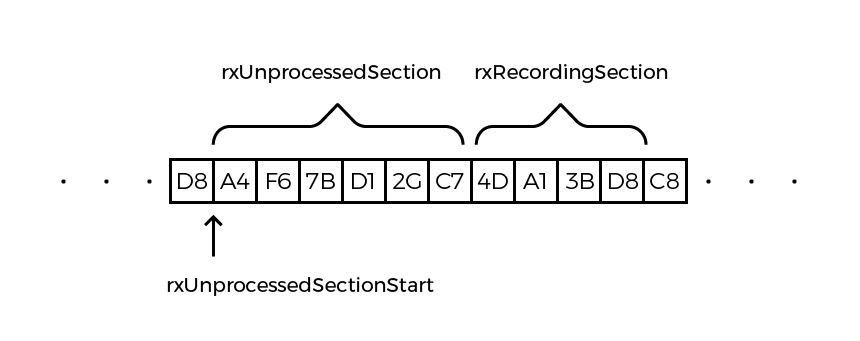
\includegraphics[width=1\textwidth]{dma-rx-buffer}
\end{center}
\caption{RX Buffer for Link Device's UART.}
\label{dma-rx-buffer}
\end{figure}

As illustrates in figure \ref{dma-rx-buffer} we only need to keep track of the start of the unprocessed section, the length of unprocessed section, and the number of bytes left to read for the DMA writing block to be finished. When the a reception finished callback called we just pass the next block to DMA channel to copy UART data into and increase the length of recording section to the block size. Of course as in the case of MACRAW socket's rx buffer, we have to perform additional procedures in the case of our next recording section reaching the end of the buffer to ensure that every frame is written in a continues block of memory.  
\chapter{RF Link}
The Link devices are communicating between each other through RF and this communication is maintained through what we call “RF Link” devices.  For this purpose, we have used the “CC1312R LaunchPad development kit” with CC1312R SimpleLink Sub-1 GHz wireless microcontroller unit. 

\begin{figure}[H]
\begin{center}
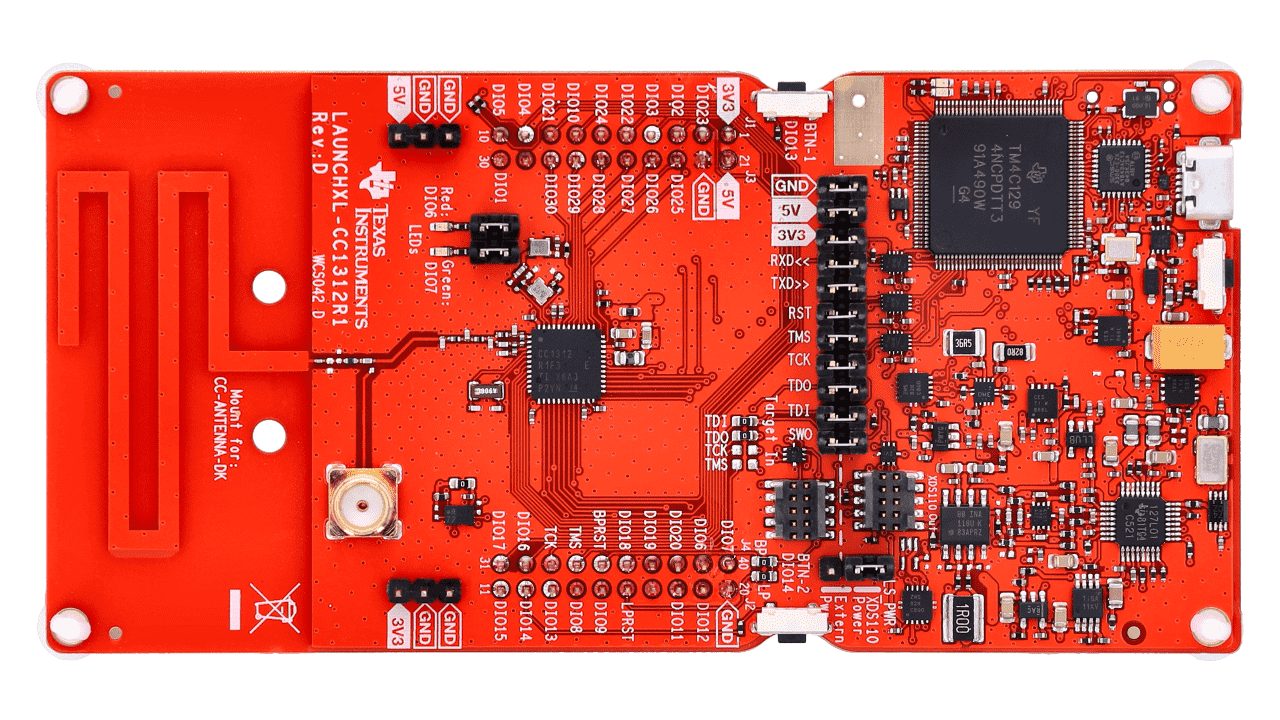
\includegraphics[width=0.90\textwidth]{cc1312r1-top}
\end{center}
\caption{Top view of CC1312R1}
\label{fig-pin}
\end{figure}

\begin{table}
\centering
\caption{Technical specifications of CC1312R1 MCU \cite{cc1312}}
\label{table1}
\begin{tabular}{|l|p{1cm}p{1cm}p{1cm}|}
\hline 
% \textbf{Name} & \textbf{Function} \tabularnewline
% \hline 
Main Processor & \multicolumn{2}{|c|}{48-MHz Arm Cortex-M4F} \tabularnewline \hline 
Programmable Flash & \multicolumn{2}{|c|}{352KB} \tabularnewline \hline 
ROM for protocols and library functions & \multicolumn{2}{|c|}{256KB} \tabularnewline \hline 
SRAM cache & \multicolumn{2}{|c|}{8KB} \tabularnewline \hline 
Ultra-low leakage SRAM & \multicolumn{2}{|c|}{80KB} \tabularnewline \hline 
\multicolumn{3}{|c|}{ Flexible high-performance sub-1 GHz RF transceiver } \tabularnewline \hline 
RF coprocessor & \multicolumn{2}{|c|}{Arm Cortex-M0} \tabularnewline \hline 
Separate SRAM & \multicolumn{2}{|c|}{16KB} \tabularnewline \hline
\multirow{3}{*}{Frequency Bands} & \multicolumn{2}{|c|}{143 MHz to 176 MHz}  \tabularnewline
{} &  \multicolumn{2}{|c|}{359 MHz to 527 MHz} \tabularnewline 
{} &  \multicolumn{2}{|c|}{861 MHz to 1054 MHz} \tabularnewline \hline
Sampling Rates & \multicolumn{2}{|c|}{2.5 kbps to 1000 kbps} \tabularnewline \hline 
Modulation Type & \multicolumn{2}{|c|}{2-FSK, 2-GFSK} \tabularnewline \hline 
\multirow{3}{*}{Receiver sensitivity} & \multicolumn{1}{|c|}{2.5 kbps (Long Range Mode)} &  \multicolumn{1}{|c|}{-121 dBm} \tabularnewline 
{} & \multicolumn{1}{|c|}{50 kbps} & \multicolumn{1}{|c|}{-110 dBm} \tabularnewline
{} & \multicolumn{1}{|c|}{1000 kbps} & \multicolumn{1}{|c|}{-97 dBm} \tabularnewline \hline 
Maximum Output power & \multicolumn{2}{|c|}{+14 dBm \newline (with temperature compensation)} \tabularnewline \hline  
\end{tabular}
\end{table}

\newpage

\section{Brief Description of RF Link's Radio Configuration}

First of all, if we want to transmit data over radio, we must choose a certain modulation scheme. The best option, for the ranges we intend to support, that CC1312R supports is 2-GFSK. All the work related to the modulation is handled by the MCU’s RF Core.
Taking this into consideration, we would not go deep into its inner workings, but very briefly: Frequency-Shift Keying (FSK) is a frequency modulation scheme in which digital information is encoded on a carrier signal by periodically shifting the frequency of the carrier between several discrete frequencies. GFKS is an extension of FSK where Gaussian filter is used to reduce the abrupt changes in frequency, resulting in a continuous phase and a bandwidth-efficient signal. 2 in 2-GFSK refers to the number of tones (frequencies with certain deviation from our carrier frequency) used to encode the signal. Table \ref{rf-link-config} presents the RF characteristics selected for our application. 

\newpage

\begin{table}
\centering
\caption{RF Link Radio Configuration}
\label{rf-link-config}
\begin{tabular}{|l|l|}
\hline 
Carrier Frequency & 868 MHz \tabularnewline \hline 
Symbol Rate & 1000 kBaud \tabularnewline \hline
Modulation Format & 2-GFSK \tabularnewline \hline
Frequency Deviation & 350 kHz \tabularnewline \hline
RX Filter Bandwidth & 2185.1 \tabularnewline \hline
\end{tabular}
\end{table}

\begin{table}
\centering
\caption{RF Packet Structure}
\label{rf-pkt-struct}
\begin{tabular}{|l|l|l|l|l|}
\hline 
Preamble & Sync Word & Length Byte & Payload & CRC \tabularnewline \hline
4 bytes & 4 bytes & 1 byte & 1 - 255 bytes & 2 bytes \tabularnewline \hline
\end{tabular}
\end{table}

The preamble in the proprietary PHY consists of an alternating bit pattern 0101... and is used to determine the amplifier gain. Unlike in older TI devices, it is not needed for the bit synchronization (Cite Packet Format Documentation). 
The sync word is used by the packet engine to detect the packet start, meaning it has a similar purpose to the start delimiter in Interlink packets. The value for the sync word is selected such that it has high self-correlation. We are using the default sync word for CC1312R: 0x930B51DE.
As we are using variable length packets, the length byte is automatically added by the transmitter, so that receiver will know the number of bytes expected in the payload.
At the end of the packet CRC is added, which is used to detect when a packet is received with errors.

\section{Interaction with RF Core Coprocessor}

As it has already been mentioned the inner workings of RF Core of CC1312R MCU are abstracted away and we are interacting with it through TI’s drivers. There are 3 commands we have used:
\begin{enumerate}[nolistsep]
\item CMD\_FS - Sets frequency and start the synthesizer 
\item CMD\_PROP\_TX - Used to pass transmission related commands to the RF core 
\item CMD\_PROP\_RX - Used to pass reception related commands to the RX core 
\end{enumerate}

One important remark is that RF Core’s controller has a separate built-in RAT (Radio Timer), which is used for the accurate timing of the command execution. This timer would not be affected by the execution of our main program, which is crucial for maintaining correct timings as it will become apparent later.

The commands can be given to the RF core in various ways - the 3 most important ones being:

\begin{enumerate}[nolistsep]
\item Abort all current operations and immediately proceed to the execution of the given command,
\item Append the given command to the current execution chain to be executed after all the currently queued radio operations are finished,
\item Schedule a command to be executed with precise timing, which is given in RAT timer ticks. This one is especially important, because things like transmission operation need a “warm-up” time to reach the state when the transmission can begin. This is crucial as by scheduling a command at a precise time, the RF core processor would perform the “warm-up” beforehand to start the transmission precisely at the specified time.
\end{enumerate}

\section{Time-Division Multiple Access Configuration}

As our RF link agents have to share a communication medium (i.e., air, as we are using RF), we must employ some sort of channel access method. The method we have chosen is Time-Division Multiple Access (TDMA), where agents have dedicated time slots for transmission. In our case, we have settled on building a half-duplex communication system, where the parties can communicate bidirectionally, but not simultaneously. As currently we only have enough hardware on hand for two RF devices, we decided to organize time division in the following manner: one of the RF devices will take the role of the “master" and the other will be assigned the role of the "slave." 
The roles are assigned based on the state of the GPIO pin DIO25. This pin is operating in pull up mode, so if we connect it to ground with a jumper, the value of the pin will become 0, meaning it will be the \emph{slave}.
Based on the initialized roles, both of the agents know their designated time slots, assuming they have synchronized clocks. Moreover, we are using roles in the process of the clock synchronization as the \emph{slave} adjusts its clock based on the \emph{master’s} clock (this process will be examined in more detail later). Each time slots has a duration of 2500 microseconds, during which one of the parties will transmit and the other will receive. The time slots are virtually divided into odd and even numbers, the \emph{master} device will transmit data (if data is available) in even time slots and \emph{slave} device will transmit data in odd timeslots. As long as both devices have synchronized time slot timer (system clock), they should not transmit data at the same time (so that transmitter collision will be avoided).
\begin{figure}[H]
\begin{center}
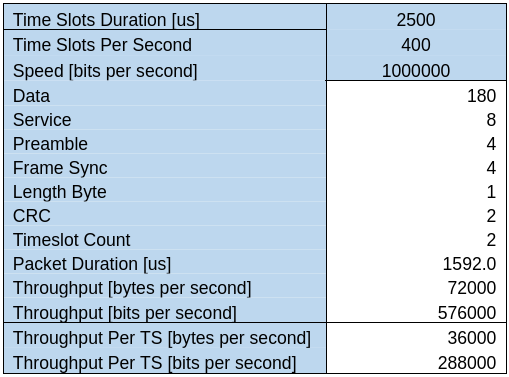
\includegraphics[width=0.60\textwidth]{TDMA}
\end{center}
\caption{TDMA Characteristics}
\label{tdma-chrac}
\end{figure}

The throughput of each timeslot is 36000 bytes per second, the UART speed (described in the section below) is 230400 bauds, which corresponds to 23040 bytes per second. As a result, the bottleneck of the system is not in the RF communication, but rather the UART link. 

\section{RF Link's Connection to Link Device}

We will communicate with the “Link device” through UART. We encountered an issue with our MCU’s UART not working properly with non-standard baud rates. The baud rate of the UART is set to 230400 bauds per second as the processing power of our chip was not sufficient to handle processing data if we increased the baud rate to the next standard value of 460800. This is unfortunate, as the throughput of our RF should have been sufficient for higher data rates, but our chip was unable to handle the processing of so much data. As in the case of the “Link device’s” UART connection, we are using DMA to offload some work from our processor. Fortunately, TI’s drivers simplify the process a lot, and the only thing left for us to do is to oscillate between the two buffers of the maximum RF packet payload size (180 bytes) on reception callback. 

\section{RF Link Timer}

At the initial boot-up of the RF link module, we start a 16 bit timer with a period of 10 microseconds. We set its interruption priority to 1 (highest possible), so we can use this as a main system clock. 
We maintain 2 tick counters (“system time tick” and “self time tick”). In the case of the \emph{master}, these 2 tick counters are equivalent, but for the \emph{slave}, “self time tick” counter is used to keep its own time, while the “system time tick” is going to be synchronized with the \emph{master’s} time to ensure that the time slot rotations are simultaneous for all parties. Moreover, during every timer interrupt callback, we check if we have reached the current device’s transmission time slot. If so, in a case of having data to be transmitted, we perform the following 3 operations:
\begin{enumerate}[nolistsep]
    \item Set a flag that indicates the need for processing an upcoming TX packet. We do not perform the processing of the upcoming TX packet at the interrupt itself, as we do not want to block the program execution flow in the interrupt,
    \item Fix the current system tick counter in the variable "txSyncTick". This is only being used in the case of the \emph{master} as it must share its time for the other parties in the network to adjust their system times according to it,
    \item Calculate the transmission start time. It is calculated as: \[ \text{Current\ RAT\ Time + TX\_CMD\_TO\_START,} \] where “TX\_CMD\_TO\_START” is the time that would be sufficient for the RF core to reach the state of readiness for transmission. Also, having a margin before the start of the packet transmission allows us to have lower time synchronization accuracy.
\end{enumerate}

\section{RF Link Packet Structure}


\begin{table}
\centering
\caption{RF Link Packet Structure}
\label{rf-link-pkt-struct}
\begin{tabular}{|p{1in}|p{1.5in}|p{2in}|} \hline 
\multirow{4}{*}{Header} & Packet type & {1 byte unsigned integer} \\ \cline{2-3}
 & Packet ID & 1 byte unsigned integer \\ \cline{2-3}
 & Payload length & 2 byte unsigned integer \\ \cline{2-3}
 & System tick value & 4 byte unsigned integer \\ \cline{2-3} \hline
 \multicolumn{2}{|c|}{Payload} & Max 180 bytes \\ \hline
\end{tabular}
\end{table}

When designing the initial structure, we have devised 2 packet types (service and data), but currently we have no use for the service packets. The same situation occurs with IDs as we do not use them either, but the IDS are intended to later be used to facilitate the ability to request the repetition of corrupted or missed packets.

\section{RF Transmission Procedure}

On every cycle of the program's execution loop, we check if any data has been received via UART and if so, we prepare a radio packet to be transmitted when the current party's transmission time slot begins. The packet is enqueued to the transmission queue, and we have its maximum length set at 10. As the speed on RF communication is higher then the speed of UART communication, this queue should never reach its maximum length. 
If during the execution loop our program encounters the flag that indicates the need for processing an upcoming TX packet being set, it performs a procedure represented by the following pseudo code:

\lstset{language=c, showstringspaces=false, tabsize=1, breaklines=true, breakatwhitespace=false, framexleftmargin=20pt,numbers=left, 
numberstyle=\small,numbersep=10pt,frame=single,captionpos=t,xleftmargin=.061\textwidth}
\begin{center}
\begin{lstlisting}[caption=RF Transmission Preperation Procedure, label=nodemcuconfig]
start_time <- RF_getCurrentTime()
fixTickCounter()
RF_cancelOngoingCommand()
txPacket <- getCurrentTXPacket()
txPacket.header.tick <- txSyncTick
RF_sendPacket(txPacket)
RF_startReception()
resumeTickCounters(RAT_TO_SYSTICK(RF_getCurrentTime() - start_time))
processTxPacketFlag <- false
\end{lstlisting}
\end{center}

The drivers that TI provides are written in such way that all interrupts are disabled during the process of passing the command to RF core. As this would mess up our tick counter, we had to come up with a workaround. The workaround consists of stopping the timer at the beginning of the procedure and at the end of the procedure resuming it after fixing the tick values using the time difference measured using the RAT, which is unaffected by disablement of interrupts as it runs on the RF core. It is carried out in the lines 1, 2, and 8. It is important to note that in the "RF\_sendPacket" sub procedure we send the transmission command to the RF core with the scheduled time calculated when \emph{processTxPacketFlag} was set. At the end, we send a new command to RF core to start reception, which would queue in the command chain, as there is no reason to stay in transmission mode after the data has been sent, i.e., the previous command for transmission had been finished executing. 

\section{RF Reception Procedure}

The TI driver for RF core provides the ability to register a callback on the data reception. We are interested in two events:
\begin{enumerate}[nolistsep]
    \item \emph{RF\_EventRxOk}: occurs when a packet reception has finished,
    \item \emph{RF\_EventRxEntryDone}: occurs when the last packet that was received is available to be read.
\end{enumerate}

In the case of the first event occurring we just fix the tick value in the “rxRdyTick” variable. In case of the second event, we read the packet from the RFQueue (provided in the TI drivers) and enqueue it in our internal rx packet queue with its “rxRdyTick”. On the next iteration of the program’s loop we send the packet’s payload to the Link device through UART. If the receiving device has the role of the \emph{slave}, it proceeds to system tick adjustment procedure.

\section{RF Synchronization Procedure}

First, we must calculate the time in ticks that has passed since we have received the packet. We do so by subtracting the “rxRdyTick” from the current value of the tick counter and store it in “rxTickPassed”. Then we calculate the packet transmission duration. Below is the formula for its calculation:

\begin{equation}
t_{packet} = \frac{(N_{preamble} + N_{syncword} + N_{length} + N_{CRC} + N_{header} + N_{payloadLength}) \times 8}{\text{Data Speed}} \times 1000000
\end{equation}

Where:
\begin{enumerate}[nolistsep]
    \item \(N_{preamble}\): number of bytes in the preamble (4 in our case),
    \item \(N_{syncword}\): number of bytes in the sync word (4 in our case),
    \item \(N_{length}\): number of bytes of the packet length field (this is automatically calculated and added by RF core) (1 in our case),
    \item \(N_{CRC}\): length of CRC in bytes  (2 in our case),
    \item \(N_{header}\): length of our packets header in bytes (8 in our case),
    \item \(N_{payloadLength}\): length of our payload in bytes (0-180 in our case),
    \item \(N_{preamble}\): number of bytes in the preamble (4 in our case),
    \item Data Speed: Symbol Rate, meaning number of symbols (in case of 2-GFSK, bits) per second (1,000,000 in our case),
\end{enumerate}

The part of the equation in the bracket is the length of the whole RF packet in bytes. We multiply it by 8 to get the number of symbols (bits). Then we divide it by "Data Speed" to get the duration of the packet in seconds and then multiply it by 1,000,000 to convert it to microseconds. After we have obtained the packet duration, we can calculate the new adjusted system tick.

\begin{multline}
\text{system tick = } tick_{rxHeader} + \frac{\operatorname{RatTicksToUs} (tick_{cmdToStart} + tick_{startToPreamble})}{N_{usInTick}} \\  + \frac{t_{packet}}{N_{usInTick}} + rxTickPassed + \frac{100}{N_{usInTick}}
\end{multline}

Where:
\begin{enumerate}[nolistsep]
    \item \(tick_{rxHeader}\): the tick value of master's system tick on its transmission slots beginning,
    \item \(tick_{cmdToStart}\): the time between the beginning of the time slot and the start of transmission in RAT ticks,
    \item \(tick_{startToPreamble}\): the time between the start of transmission process and the start of preamble being sent (the time when data physically starts to transmit),
    \item \(RatTicksToUs\): RAT ticks to microseconds conversion operation,
    \item \(N_{usInTick}\): number of microseconds in one tick. We divide by it the microseconds values to get the value in ticks.
\end{enumerate}

The last part of the equation may seem bizarre. We have found it experimentally, by looking at the difference between the clocks of \emph{master} and \emph{slave} with an oscilloscope even after adjustment. The reason for the constant error is possibly the RF signal demodulation process. This includes data demodulation, CRC calculation and copying of the data from internal buffers to the reception queue for outputting data from RF core.
It may seem unnecessary to adjust the clock on the \emph{slave} on every received packet, but it is very important because every crystal oscillator (which is used to generate the operational clock of the microcontroller, and as a result the system timer) has some inaccuracy and the inaccuracy can differ from one crystal oscillator to another and even though the inaccuracy may seem insignificant, it can add up over time causing drift between the agents' clocks if we just adjust them once.

\begin{figure}[H]
\begin{center}
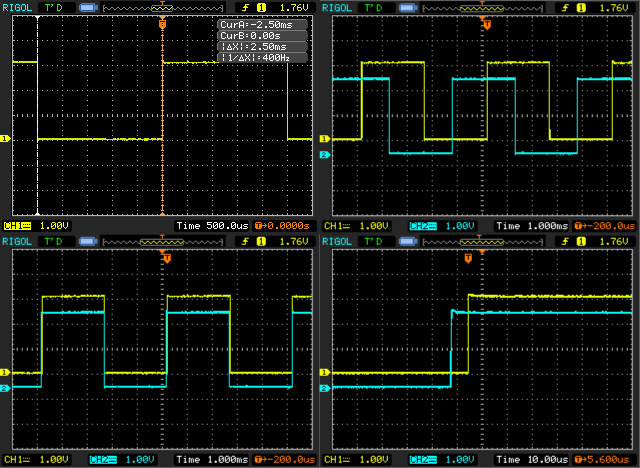
\includegraphics[width=0.90\textwidth]{time-slots.png}
\end{center}
\caption{Screenshots of oscilloscope showing the time slots, where lows are the odd time slots, and the highs are the even time slots. (top left) Measurement of the duration of single time slot. (top right) Signals from \emph{master} and \emph{slave} device before synchronisation. (bottom left) Signals from \emph{master} and \emph{slave} device after synchronisation. (bottom right) Close-up of the signals from \emph{master} and \emph{slave} device after synchronisation. }
\label{fig-oscilloscope}
\end{figure}

As it can be seen in the right bottom section of \ref{fig-oscilloscope}, even after the synchronisation, we have approximately 7 microseconds of discrepancy between clocks. This is expected as timers on RF Links run with 10 microseconds period, so our error theoretically can't be lower then that. However, even with this 10 microseconds of error, our synchronisation procedure yields results that are more than sufficient to maintain a reliable operation of our system.  


% The NodeMCU parameters are listed in Table \ref{table2}.

% \begin{table}
% \caption{Parameters of NodeMCU}
% \label{table2}
% \centering
% \begin{tabular}{|l|p{3.7cm}|p{4.8cm}|}
% \hline 
% \textbf{Categories} & \textbf{Items} & \textbf{Values} \tabularnewline
% \hline 
% \multirow{1}{*}{Wi-Fi Parameters} & certificates & FCC/CE/TELEC/SRRC \\\cline{2-3}
%                  & WiFi Protocols & 802.11 b/g/n \\\cline{2-3}
%                  & Frequency Range	 & 2.4G-2.5G (2400M-2483.5M) \\\cline{2-3}
%                  & \multirow{2}{*}{TX Power} & 802.11 b: +20 dBm \\\cline{3-3}
%                  & & 802.11 g: +17 dBm \\ \cline{3-3}
%                  & & 802.11 n: +14 dBm \\ \cline{2-3}
%                  & \multirow{2}{*}{RX Sensitivity} & 802.11 b: -91 dbm (11 Mbps)   \\\cline{3-3}
%                  & & 802.11 g: -75 dbm (54 Mbps)  \\ \cline{3-3}
%                  & & 802.11 n: -72 dbm (MCS7) \\ \cline{2-3}
%                    & Types of Antenna & PCB Trace, External, IPEX Connector, Ceramic Chip    \\ \cline{1-3}
                 
% \multirow{1}{*}{Hardware Parameters} & \multirow{2}{*}{TX Power} & UART/SDIO/SPI/I2C/ \newline I2S/IR Remote Control \\\cline{3-3}
%                  &  & GPIO/PWM\\\cline{2-3}                
%                  & Operating Voltage & 3.0~3.6V \\ \cline{2-3}
%                  & Operating Current & Average value: 80mA \\ \cline{2-3}
%                  & Operating Temperature Range& -40°~125° \\ \cline{2-3}
%                  & Ambient Temperature Range & Normal temperature  \\\cline{2-3}
%                  & Package Size & 5x5mm  \\ \cline{2-3}
%                  & External Interface & N/A \\ \cline{1-3} \hline 
% \end{tabular}
% \end{table}

\chapter{Conclusion}

To test the real world performance, we have connected computers to both agents of our system and hosted an Updog (a small program that allows uploading and downloading files via HTTP/S) server on one of them and loaded a page on other computers browser.

\begin{figure}[H]
\begin{center}
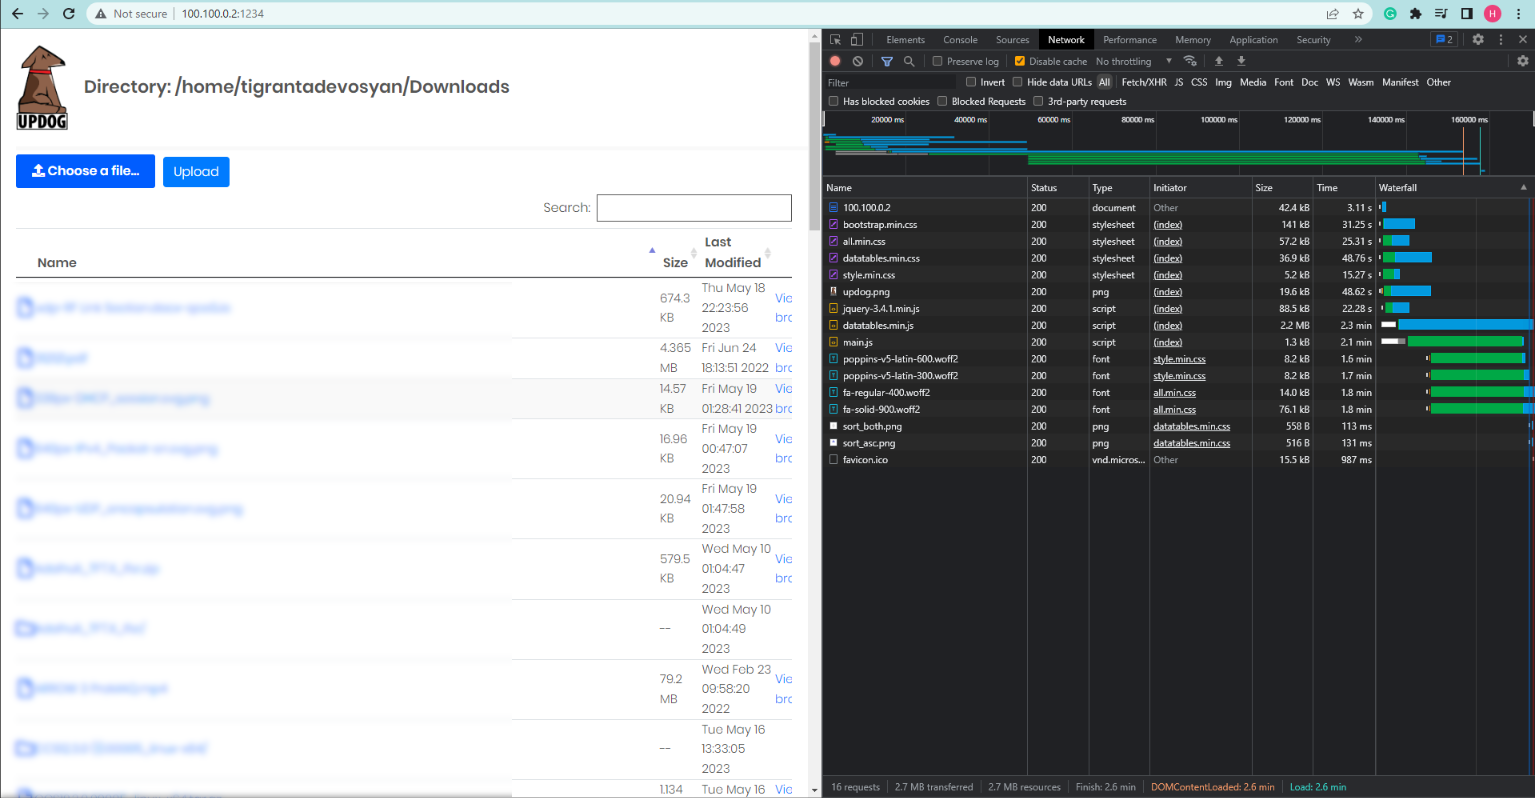
\includegraphics[width=0.90\textwidth]{updog-2.png}
\end{center}
\caption{Screenshot of Updog loaded through our network.}
\label{updog}
\end{figure}

A 2.7 Mb was loaded in 2.6 minutes, which means we had average data speed of 17.3 KB/s. Of course this is not representative of the throughput of the system as 2.7 Mb is just the amount that was finally loaded and there is other traffic going around that is not included 2.7 Mb (for example acknowledgment messages). Moreover, there are going to be some packets that become corrupted during transmission or fragments of the are dropped as the system is overloaded. But in our opinion this metric is more important as it represents the real world capabilities of the system.   

\begin{figure}[H]
\begin{center}
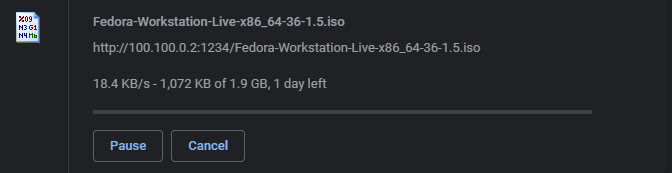
\includegraphics[width=0.90\textwidth]{download.png}
\end{center}
\caption{Screenshot of download a file through our network.}
\label{download}
\end{figure}

Above is a figure of file download process through our system and as it can bee seen, we are able to maintain approximately 18 KB/s of sustained traffic. Of course the is not enough to things that we are accustomed to do through Internet, like streaming an HD video, but it would be more then enough to accommodate file transfer in cases when wired connection is inconvenient or impossible (for example a UAV during flight). Moreover, with the help of modern compression algorithms the throughput is more then enough to facilitate a relatively decent voice streaming. For application where the data rate is low, like text messaging, the system can be used to connect subnetworks with multiple users to each other. 

As it have already been mentioned the main "bottle-neck" for our system's throughput turned out to be the processing power of the RF link. One possible method of increasing it is the optimizing of the source code of the RF link, but the gains that can be achieved this ways are relatively insignificant. A more realistic way would be changing the hardware of the RF link, as a faster MCU would significantly increase the throughput of the system up until other parts of the system become the "bottle-neck". Integration of the system on one circuit would allow us to increase the stability and speed of SPI and UART connections. Moreover, we can increase the Ethernet reception and transmission, by replacing the W5500 with Microchip's first party ETHERNETPHY module.

With the help of Free Space Path Loss equation we have calculated that maximum theoretical distance our radio can work for our maximum output power (+14 dBM) is 12km. Obviously in real world application the maximum range would be closer to 10 km assuming good conditions like relatively low noise in the environment and unobstructed vision. There are three main ways of increasing the maximum operational range: 
\begin{itemize}[nolistsep]
    \item Improving transmission by connecting an external power amplifier,
    \item Using external high gain antennas, 
    \item Improving reception with low noise amplifiers on receiver.
\end{itemize}

Other improvements might be:
\begin{itemize}[nolistsep]
    \item Dynamic assignment of roles and time slots and facilitation of more agents in the network,
    \item Use of multiple antennas to achieve a full-duplex communication or increas overall system throughput in the case of high number of agnets in the network, 
    \item Integration of the system into a complete package, by designing a custom PCB, case, and battery.
\end{itemize}

\begin{figure}[H]
\begin{center}
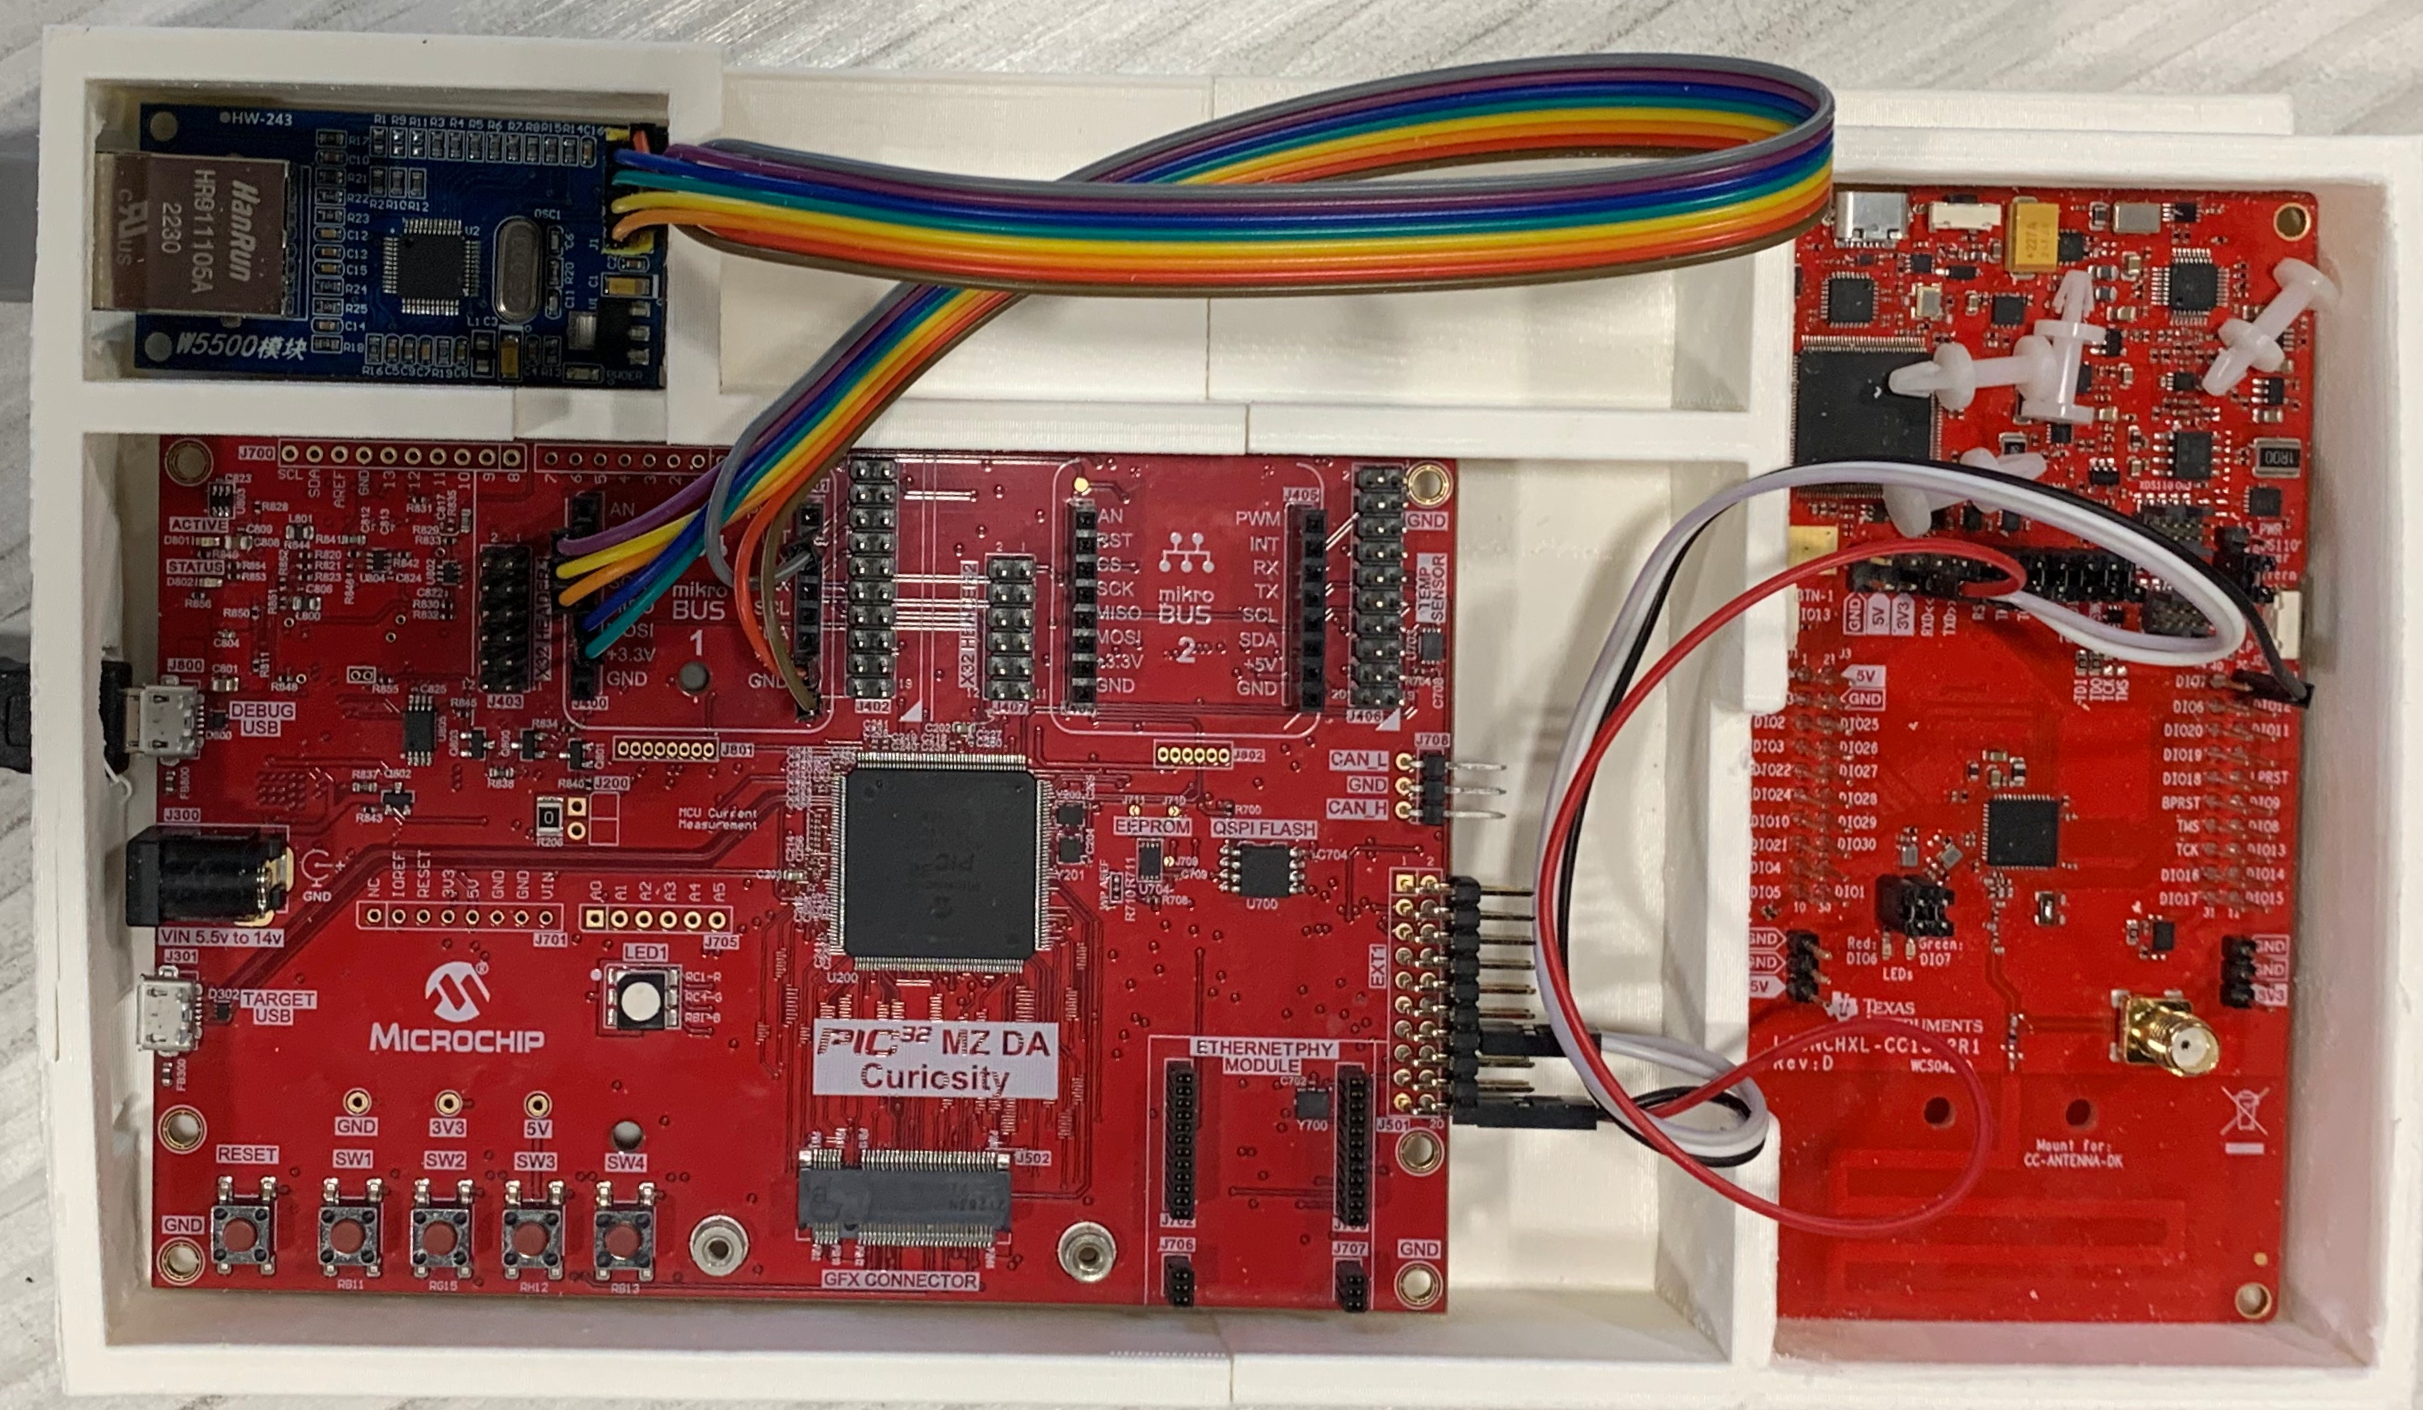
\includegraphics[width=0.90\textwidth]{final.jpg}
\end{center}
\caption{Final result.}
\label{download}
\end{figure}




%\bibliographystyle{plainnat}
%\bibliographystyle{IEEEtran}
\bibliographystyle{IEEEtranN}
\bibliography{references}


\appendix
% \include{appendix}

\newpage{}

\end{document}